\documentclass[12]{report}
\usepackage{graphicx} % Required for inserting images
\usepackage[top=2cm,bottom=2cm,left=1.2cm,right=1.2cm,marginparwidth=1.75cm]{geometry}
\usepackage{amsmath}
\usepackage{setspace}
\usepackage{float}
\usepackage{amsmath}
\usepackage{natbib}
\usepackage{nccmath}
\usepackage{hyperref}
\onehalfspacing
\usepackage{booktabs}

\begin{document}
\begin{titlepage}
    \centering
    \vspace*{1cm}
    \begin{spacing}{2}
    \textbf{\Huge Exploring the Impact of Lighting Conditions on Injury Severity in Single Vehicle Collisions Utilizing  Zero-Inflated Ordered Probit Model}
    \end{spacing}
    
    \vspace{1cm}
    
    {\Large 
    Ifeanyi Omeifejideofor \\
    \vspace{0.5cm}
    
    \textbf{School of Mathematics and Statistics} \\
     \vspace{0.5cm}
     
    \textbf{The University of St Andrews} \\
     \vspace{0.5cm}
     
    August 2023 \\
     \vspace{0.5cm}
    Supervised by }
    
    \vfill

    {\large 
    \textit{
    I hereby certify that this dissertation, which is approximately . . . words in length, has been composed by me, that it is the record of work carried out by me, and that it has not been submitted in any previous application for a degree. This project was conducted by me at the University of St Andrews from [month/year] to [month/year] towards the fulfillment of the requirements of the University of St Andrews for the degree of [insert name] under the supervision of [insert signature].
    }}

    \vfill

\end{titlepage}



\chapter{Introduction}

\chapter{Literature Review}

\chapter{Data Exploration}
\section{Data Description}
\begin{quote}
{\large 

Over the years documenting and reviewing traffic-related incidents has become crucial for public safety policies, city planning, and infrastructure investments in countries. The United Kingdom is no exception, as it strives to improve road safety by implementing the STATS19 data collection system. The STATS19 database is a standardized police crash report of all road traffic accidents that resulted in personal injury (Department for Transport); it is essential for conducting studies and gaining insights into the complex dynamics of road safety. Researchers use statistical and machine learning methods to analyze this dataset thereby uncovering connections between different variables, identifying patterns, and understanding the underlying relationships that influence accident outcomes. However, the dataset records injury-only accidents and this limits the dataset scope, as accidents without injuries are not captured in the records(Imprialou and Quddus, 2019).

The STATS19 dataset measures injury severity using three distinct classification methods, which are slight, severe, and fatal. However, these classifications are similar to the KABCO scale, commonly used by professionals in road safety and accident analysis, which categorizes injury severity as non-capacitating, incapacitating, and fatal. The STATS19  dataset contains  layers of information related to various accident scenarios. These can be categorized into details concerning casualties, vehicle-related information, pedestrian-related information, environmental factors, and all road information. 

To explore in-depth, the accident data consist of vehicle-related information, such as maneuverability, skidding and overturning, point of impact, and vehicle age. Additionally, the dataset records the vehicle's location during the accident, indicating whether the vehicle was in the carriageway or off the carriageway.

Moving to casualty-related information, the dataset includes information such as casualty severity, age of casualty, and details relating to pedestrian involvement. This includes pedestrian location, pedestrian movement, whether pedestrian
were road maintenance workers.

\clearpage
Environmental factors are essential in determining the dynamics of an accident (Grigorios et
al., 2020); the dataset records essential environmental variables at the time of the accident, such as weather conditions and lighting conditions.

Finally, the dataset captures all other essential variables which are pivotal in determining the dynamic of an accident, such as speed limit, junction details, road types, road class, junction control, carriageway hazards, and urban or rural areas. These variables provide an exhaustive list of contributory factors essential for understanding injury severity.
}
\end{quote}


\section{Data Preparation}
\begin{quote}
{\large
The STATS19 dataset containing accident information from 2016 - 2021 was used for this analysis, and it includes accident data, vehicle, and casualty information within the five-year period. The accident data contains 562,439 observations, casualties 728,541 observations, while the vehicle data contains 1,034,534 observations. However, the researcher noticed that the higher count of observations in the casualties and vehicle data resulted from the presence of duplicated values.
The duplicates in the vehicle data were caused by accidents involving more than one vehicle; therefore, to address the duplicated instances in the vehicle data, only accidents or collision involving a single vehicle was chosen for this analysis. Additionally, to account for the duplicated values in the casualty data, the approach taken was to select the highest casualty severity value. This decision was motivated by cases where duplicates occurred due to accidents involving multiple individuals. The files were linked together using the accident index variable, which is common across all three distinct files. The combined dataset was cleaned to ensure accuracy and reliability utilizing statistical and industry knowledge.

One aspect of the cleaning process involves the removal of negative values. These negative values do not exist in the current encoding of STATS19 accident values, which was done for all columns in the combined dataset. To enhance the dataset consistency and mitigate the introduction of bias in the model, encoding representing unknown values was removed from  columns like drivers' sex, weather conditions, and road types For example, encoding such as 'unknown driver sex' was used to depict hit-and-run accidents where police could not trace the driver. Studies have shown that hit and run accidents involved pedestrians, and factors like drinking and driving were some of the key reasons why hit and run drivers left the scene as their decision-making became impaired (Hopkins et al., 2017).

Additionally, variables that do not contribute to driving the research were removed, including accident reference, casualty reference, if a police officer attended the scene of the accidents, home area type, etc. Accidents involving pedestrians, and pedal cyclists were also excluded from the model because pedestrians have different injury mechanisms (Jiang et al., 2013). To elaborate further, pedestrians are vulnerable and exposed, thus, lacking the protection that a vehicle provides for its occupants hence accidents involving pedestrians might lead to a higher and different injury severity compared to vehicle passengers.

Furthermore, intersection-related variables were excluded because intersections involve complex interactions as vehicles, pedestrians, and cyclists cross paths in different directions. This leads to different types and patterns of accidents compared to those on continuous road segments where the movement is largely in one direction. Large trucks, coach buses,  and non-traditional vehicles were also excluded from the dataset because their size and weight subject them to varying accident types, and the injury mechanism differs in these vehicles.

\begin{figure}[H]
    \centering
    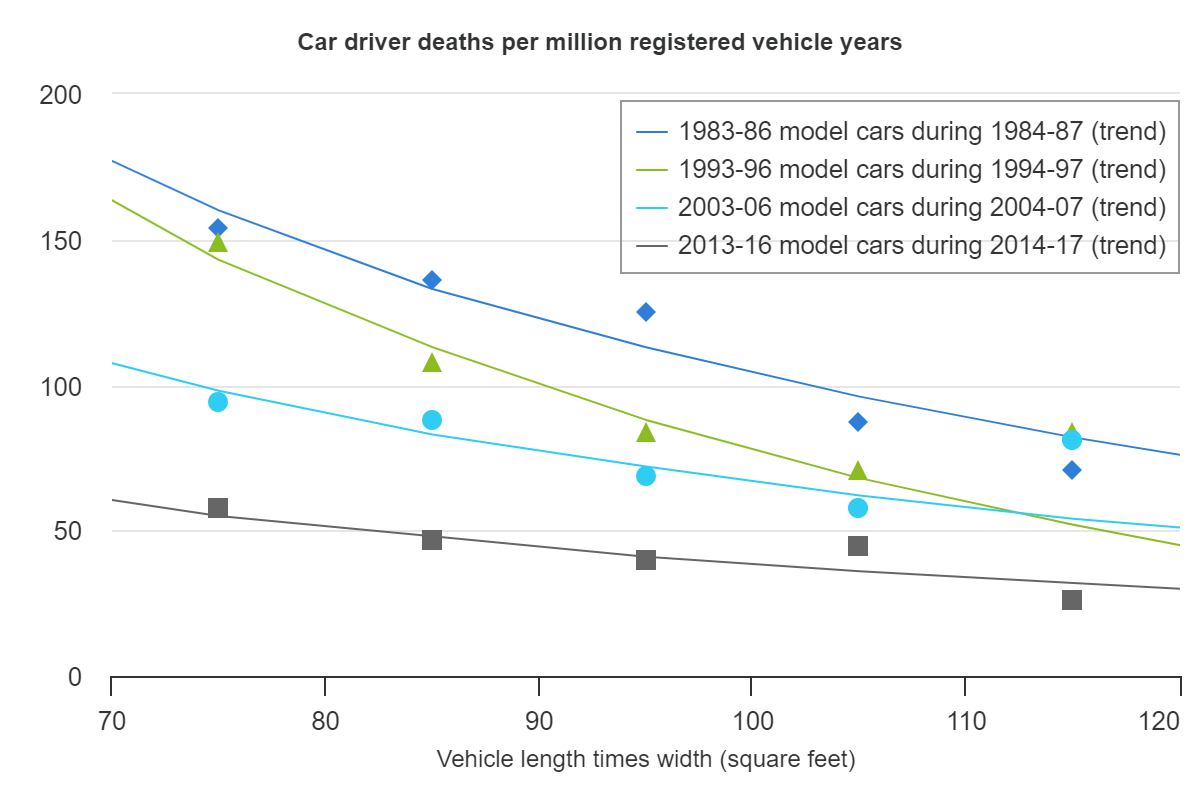
\includegraphics[width=0.8\textwidth,keepaspectratio]{Figs/car-driver-deaths-per-mi.png}
    \caption{source: Insurance Institute for Highway Safety(IIHS)}
    \label{fig:enter-label}
\end{figure}

An illustration of this difference in injury mechanism can be observed in Figure 3.1, where crash deaths decline as vehicle size increases. According to the insurance institute for highway safety(IIHS), larger vehicles offer better protection for occupants because the part of the vehicle between the front bumper and the occupant compartment absorbs energy from crashes by crumpling. As a result, longer front ends offer better protection in frontal crashes. Heavier vehicles also tend to continue moving forward in crashes with lighter vehicles and other obstacles, so the people inside them are subject to less force. Additionally, motorcycles and other non-conventional vehicles were excluded due to their limited representation within the dataset.

The vehicle age was also restricted to a maximum of 24 years due to the evolution of safety regulations and advancements in car safety standards. This is because cars within this range share similar safety features such as airbags, seat belts, and whiplash systems which have become standard for auto manufacturers. 

\clearpage
The Pearson correlation coefficient was calculated to avoid the potential issue of multicollinearity between the variables, as strong correlations could lead to instability in the parameter estimates and inflated standard errors, hence causing difficulties in discerning the effect of each individual predictor. A threshold of 70 percent was set to determine the correlation. Correlation coefficients falling  between 70  and 90 percent
indicates a high correlation.

\begin{figure}[H]
    \centering
    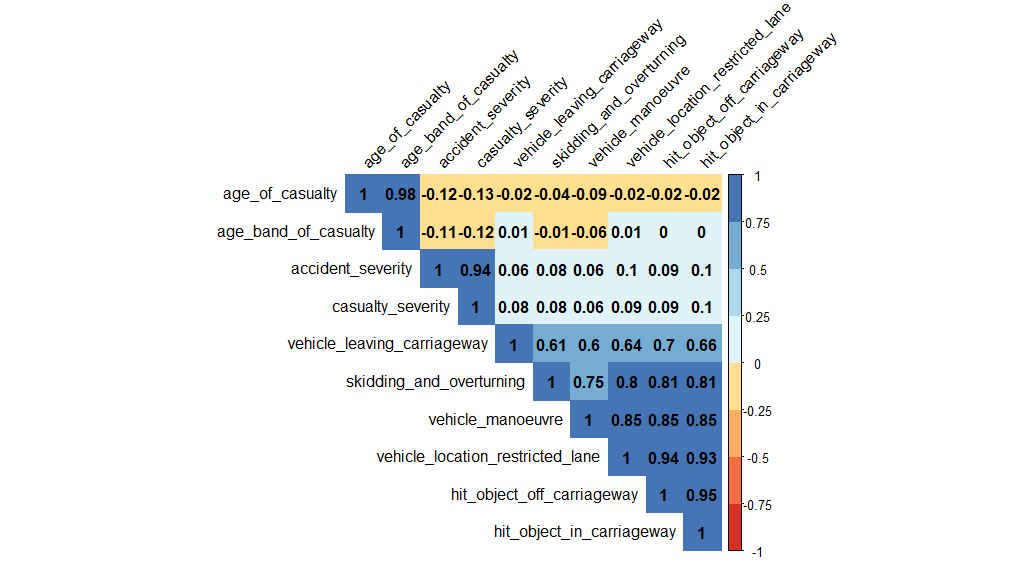
\includegraphics[width=0.8\textwidth,keepaspectratio]{Figs/correlation_updated_new.png}
    \caption{ Variable Correlations}
    \label{fig:enter-label}
\end{figure}

In Figure 3.2, a group of highly correlated variables can be observed. However, certain variables were omitted from the model to address multicollinearity and reliability of the model. Variables such as hit objects off the carriageway, vehicle location restricted lane, and vehicles leaving the carriageway were excluded; the exclusion of these variables was not limited to their significant correlation but also because their impact on injury severity may be less related to lighting conditions and more influenced by other factors such as driver behavior, distractions and more. This is consistent with studies (McLaughlin et al., 2009) that highlight how accidents involving vehicles leaving the carriageway are often caused by distracted drivers.

Additionally, variables sharing similarities, such as accident severity and age band of casualty, which are closely linked to severity of casualty and age, were excluded;  hit objects in the carriageway and vehicle maneuvers were removed to reduce the effect of collinearity in the model. The final dataset used for model estimation includes 16,821 observations of single-vehicle collisions. In terms of injury severity, slight injury accounted for  74.55\%  of collisions, severe injury accounted for 23.95\%, and fatal injury constituted 1.49\%  of collision injury severity.

\clearpage
Figures 3.3 and 3.4 depict the variations in injury severity and its distribution across different lighting conditions. The collision data consistently exhibit a higher frequency of slight injuries. This distribution pattern might suggest the possibility of underlying injury severity patterns influencing the mechanism of collision occurrence.

\begin{figure}[H]
    \centering
    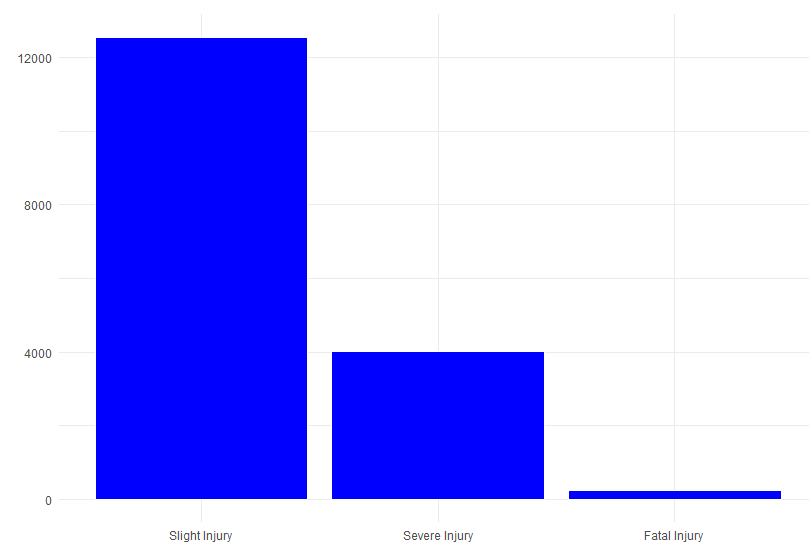
\includegraphics[width=0.65\textwidth,keepaspectratio]{Figs/histogram_ziop.png}
    \caption{ Histogram of Injury Severity}
\end{figure}

\begin{figure}[H]
    \centering
    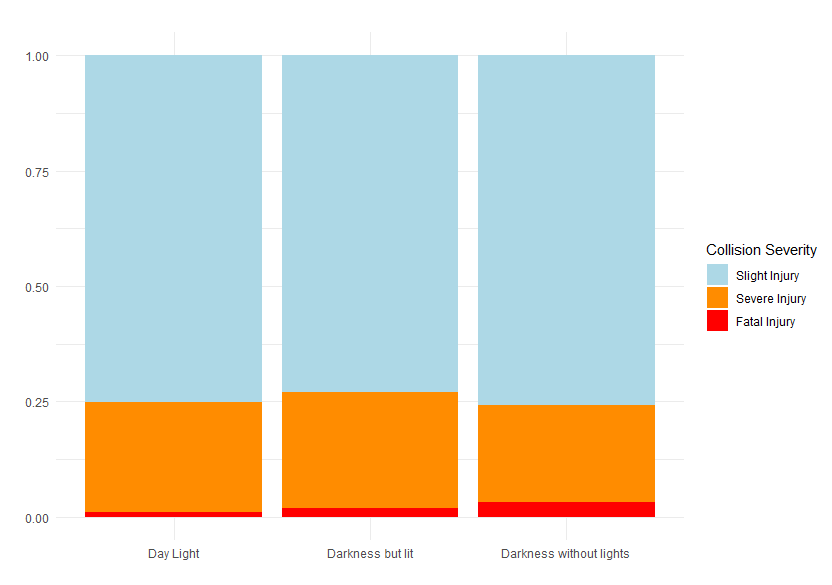
\includegraphics[width=0.65\textwidth,keepaspectratio]{Figs/collision_severity.png}
    \caption{Histogram of Injury Severity Distribution across various Lighting Conditions}
\end{figure}

\clearpage
The collision data used for this research contains an exhaustive list of information. They are summarized and presented in Table 3.1 below:
\vspace{0.04cm}

\begin{table}[H]
\renewcommand{\arraystretch}{1.06}
\centering
\begin{tabular}{p{4cm} p{8cm} c c c}
\toprule
\multicolumn{5}{c}{Table 3.1: Variable Descriptions and Summary Statistics} \\
\midrule
Variable & Description & Mean or \% of 1 & Min & Max \\ 
\midrule
Road type indicator & 1 if collision occurred on a carriageway, 0 otherwise & 93.13\% & 0 & 1 \\

Speed limit indicator & 1 if the speed limit is above 40 mph, 0 otherwise & 14.22\% & 0 & 1 \\

Weather condition indicator & 1 if collision occurred in fine weather, 0 otherwise & 81.72\% & 0 & 1 \\

Road surface conditions indicator & 1 if collision occurred in wet roads, 0 otherwise & 29.98\% & 0 & 1 \\

Special conditions at site indicator & 1 if road hazards present (Debris present, Defective Road), 0 otherwise & 1.68\% & 0 & 1 \\

Carriageway hazard indicator & 1 if collision involves carriageway hazards, 0 otherwise & 2.68\% & 0 & 1 \\

Urban or Rural area indicator & 1 if the collision occurred in a rural area, 0 otherwise & 16.74\% & 0 & 1 \\

Vehicle type indicator & 1 if collision involved buses and vans under 3.5 tonnes, 0 otherwise & 7\% & 0 & 1 \\

Skidding and Overturning indicator & 1 if vehicle skidded, overturned, and jackknifed during the collision, 0 otherwise & 11.59\% & 0 & 1 \\

Point of impact indicator & 1 if the vehicle was impacted (front, back, and side), 0 otherwise & 96.96\% & 0 & 1 \\

Journey purpose of driver indicator & 1 if collision is work related, 0 otherwise & 26.58\% & 0 & 1 \\

Sex of driver indicator & 1 if the driver is female, 0 otherwise & 32.25\% & 0 & 1 \\

Age of driver indicator & 1 if the driver was younger than 23 years, 0 otherwise & 18.55\% & 0 & 1 \\

Age of vehicle indicator & 1 if the age of the vehicle is less than 10 years, 0 otherwise & 35.24\% & 0 & 1 \\

Sex of casualty indicator & 1 if the casualty is female, 0 otherwise & 44.4\% & 0 & 1 \\

Age of casualty indicator & 1 if casualty age is younger than 30 years, 0 otherwise & 46.33\% & 0 & 1 \\

Car passenger indicator & 1 if collision involved a passenger car (front or rear seat), 0 otherwise & 4.51\% & 0 & 1 \\
\bottomrule
\end{tabular}
\end{table}


The use of an indicator variable allows for the comparison of groups within a categorical variable. The coefficient associated with an indicator variable provides an estimate of the average difference in the dependent variable between the groups identified by the indicator variable and reference group after taking into account other variables in the model. The reference group consists of observations where the indicator variable is always zero. In the zero-inflated ordered probit model, they represent categorical or binary variables however this method also transforms qualitative data into a format suitable for statistical analysis.  By representing these variables as indicators the model can include their impact on the outcome variable while preserving the structure required for the modeling process.
}
\end{quote}


\chapter{Methodology}
\section{Brief Description}
\begin{quote}
{\large 
This section provides an overview of the standard ordered probit model and the  zero-inflated ordered probit model(ZIOP) in addressing the critical issue of modeling a zero-inflated collision severity. It explains the underlying framework of the model and covers aspects of model evaluation and test of model fitness.}\end{quote}


\section{Standard Ordered Probit Model}
\begin{quote}
{\large 

The ordered probit model is a statistical model that handles ordinal categorical variables, it has been widely used in the analysis of traffic-related incidents and collision injury severity.  

The structure of the model can be described as follows: (Washington et al., 2003)

\begin{flalign}
r_i^* = \beta x_i + \epsilon_i \, , &&
\tag{4.2.1}
\end{flalign}

Where \(r_i^*\) is a latent variable determining the injury severity of a collision event involving a victim, \(x_i\) represents a vector of the observed explanatory variables, \(\beta\) represents the estimated parameters, and \(\epsilon_i\) is the random error term that follows a standard normal distribution.

The latent variable \(r_i^*\) is unobserved, to account for this, an observable variable \(y_i\) is introduced depicting the injury severity which can be expressed as follows: (O'Donnell and Connor, 1999)

\begin{fleqn}
\begin{align*}
{yi} =
\begin{cases}
0 & \text{if } r_i^* \leq \mu_0  \\
1 & \text{if } \mu_0 < r_i^* \leq \mu_1  \\
2 & \text{if } r_i^* > \mu_1 \, ,
\tag{4.2.2}
\end{cases} 
\end{align*}
\end{fleqn}

Here, $\mu$ represents the threshold for each severity level of injury; essentially, it denotes the  boundaries that define \(y_i\). The threshold values adhere to constraints such as $\mu_0 \leq \mu_1 \leq \mu_2 \leq \ldots \leq \mu_j$, where $\mu_j$ is the maximum ordered threshold value which corresponds to the highest injury severity level.

The probability that a collision results in an injury severity $j$ is equal to the probability that the latent variable \(r_i^*\) falls within a range defined by two thresholds. To illustrate further, provided the value of $x_i$ the probability associated with each severity level can be expressed as follows:

\begin{fleqn}
\begin{align*}
Pr(y = j) = \Phi(u_{j} - \beta x_i) - \Phi(u_{j+1} - \beta x_i)
\tag{4.2.3}
\end{align*}
\end{fleqn}

here $\Phi$ represents the cumulative normal distribution function, $u_{j}$ and $u_{j+1}$ represents the lower and upper threshold for the injury severity level.

}\end{quote}

\section{Limitation of the Ordered Probit Model}
\begin{quote}
{\large 
The standard ordered probit model is quite effective, in handling the nature of the data as it takes into account the varying levels of injury severity. However, one major criticism of this model is that it has a limited capacity in explaining the abundance of an inflated  injury severity variable especially when this variable is generated from two this distinct sources. However, this is because it assumes a uniform severity function for all types of injuries. This oversimplified assumption can lead to an inaccurate representation of the complexities within the data, potentially limiting the model's ability to accurately predict and explain injury severity across the various types of injuries.

}\end{quote}


\section{Zero-Inflated Ordered Probit Model}
\begin{quote}
{\large 

This research utilizes the zero-inflated ordered probit model(ZIOP) to address the limitations of the standard ordered probit model when analyzing accident-related data; however, this is because accident data contains an overwhelming case of zero inflation such cases could be likened to near-misses  or when safety measures prevent serious outcomes hence creating an excessive amount of zeros which presents a substantial challenge for researchers as conventional models struggle with this imbalance. 

The concept of zero inflation originates from the Poisson model of count data being overdispersed by zeros (Lambert, 1992). The zero-inflated ordered probit model(ZIOP) was developed by Harries and Zhao(2007) as an extension to the standard ordered probit model, the model accounts for the possibility of zeros generated from two distinct sources. The generation of zeros from the two separate sources causes an abundance of zeros in the dataset, leading to the term zero-inflated. The ZIOP model utilizes a double hurdle structure which consists of the binary split and ordered probit, the binary split, often referred to as the first level of the model, distinguishes between observations whose outcome is always fixed and those that follow the ordered probit process, while the ordered probit or the second level of the model estimates the probabilities of the different ordinal outcomes.

In this research, the researcher relied on the STATS19 dataset, derived from the standardized police crash reports (Department for Transport, 2022), which records injury-only accidents. A large portion of the injury data comprises of slight injuries; this accounts for roughly over 74 percent of injuries reported. This imbalance suggests the underlying process generating injuries may not be uniform and could originate from two sources. The standard ordered probit model can account for the ordinal nature of the data, but it assumes a consistent severity function across all types of injuries. However, this assumption becomes problematic and may result in biased estimates. To address the excessive presence of slight injuries and explore sub-groups within the data, a zero-inflated ordered probit model is recommended.
This approach allows for an understanding of the hidden heterogeneity in the generation process, thus providing a more accurate analysis of the injury severity levels. 

The police crash report is often prone to inaccurate classification and under-reporting of accident instances and injury severity; many slight or non-fatal injuries are not reported to the police, as this is evident in hospital records, surveys, and compensation claims data, which show relatively higher injury numbers than those documented in the police accident report (Department for Transport, 2022). Previous studies have demonstrated that accident severity can often be over- and under-classified. These results were obtained by comparing the data from hospital records with that of police reports. It was found that 19.3 percent of cases involving victims who needed to be hospitalized for longer than 12 hours (a situation usually associated with a severe injury) had incorrectly been classified in the police records as slight injuries. Alternatively, police report misclassified 9.7 percent of victims as having serious injuries despite spending less than 12 hours in the hospital, which is often suggestive of slight injuries (Tsui et al., 2008). 

The two distinct populations of accidents could explain the excessive representation of slight injuries in the data. The zero-inflated ordered probit model(ZIOP) excels in handling these types of data by utilizing its double hurdle structure, which considers two underlying states, The first state - A minor injury state that can be formed by minor collisions with less severe consequences(minor or possible injuries), This could be likened to minor accidents or collisions where damage upon impact is very low, resulting in minor injuries. As an illustration, consider the following scenario when a vehicle bumps into a small stationary object at a slow speed, The energy released upon impact is low. Hence, occupants may not sustain injuries, and even if there is a chance of injury, it would likely be extremely minor, however, recorded under the category of slight injuries (Grigorios et al., 2020; Fountas and Rye, 2019). The second state - The ordered injury state, is concerned with slight injury accidents that could lead to more severe consequences(more severe injuries) under certain unfavorable conditions, Building upon the aforementioned illustration, consider a similar scenario where the vehicle bumps into a larger stationary object at slow speed, making the impact much more significant hence could lead to more severe injuries. The ordered probit state also accounts for serious and fatal injuries (Grigorios et al., 2020; Fountas and Rye, 2019).

\begin{figure}[H]
    \centering
    \includegraphics[width=\textwidth,keepaspectratio]{Figs/ZIOPZIOPC_this.png}
    \caption{A sketch of the zero-inflated ordered probit model}
    \label{fig:enter-label}
\end{figure}

\section{Components of the Zero-inflated ordered Probit(ZIOP)}

The following describes the components of the zero-inflated ordered probit model
(Harris and Zhao, 2007). Let's denote a binary variable indicating a split in the first level of the ZIOP model where  $g_i$ = 1 (accident associated with minor injuries) and $g_i$ = 0 (accidents that do not result in minor injuries) 
\begin{flalign}
{g_i^*} = ax + \varepsilon \, , &&
\tag{4.3.1}
\end{flalign}

where \(g_i^*\) is a latent variable that indicates the propensity of an accident i to be associated with the minor injury state and \(g_i\) is derived from the latent variable \(g_i^*\), \(x\) represents a vector of determinants for the choice between both states in the binary split, \(a\) represents the vector of parameter estimates, and \(\varepsilon\) represents an error term that follows a standard normal distribution. 

The probability of being in an accident that does not result in a minor injury is  
\begin{flalign}
Pr(g_i = 0 | X) = Pr({g_i^*} \leq 0 | X) = 1-\Phi(ax) \, , &&
\tag{4.3.2}
\end{flalign}

here \(\Phi\) represents the cumulative distribution function (CDF) of the standard normal distribution. To determine factors influencing the severity of injuries resulting from accidents in the ordered probit category which is conditional on \(g_i\) = 0, the  injury level  \( \tilde{y} \) (\( \tilde{y} \) = 0,1,\ldots,J) is connected to a latent variable \(y^*\) through the ordered probit regression function:

\begin{flalign}
y^*= w\gamma + u  \, , &&
\tag{4.3.3}
\end{flalign}


where $w$ is a set of unknown parameters representing the variables influencing the frequency of non-minor injury levels, $\gamma$ represents explanatory variables in the non-minor injury state, and $u$ refers to a standard normally distributed error term independent of $\varepsilon$.

The mapping between \(y^*\) and  \( \tilde{y} \) is obtained by

\begin{fleqn}
\begin{align*}
\tilde{y} =
\begin{cases}
0 & \text{if } y^* \leq \mu_0 \\
1 & \text{if } \mu_0 < y^* \leq \mu_1 \\
2 & \text{if } y^* > \mu_1 \, ,
\tag{4.3.4}
\end{cases} 
\end{align*}
\end{fleqn}

where $\mu$ represents the threshold for each severity level of injury; essentially, it denotes the calculated boundaries partitioning the underlying latent response variable $y^*$. The threshold values adhere to constraints such as $\mu_0 \leq \mu_1 \leq \mu_2 \leq \ldots \leq \mu_j$, where $\mu_j$ is the maximum ordered threshold value.

\vspace{0.1cm}

The ordered probit state allows for a minor injury level(i.e., accident associated with minor injury or even lower severity e.g., possible injuries), and there is no requirement that xi = $\gamma_i$ hence allowing for a separate explanatory variable to be used in both part of the model. The probability of each injury level in the ordered probit states is given as:
\begin{flalign*}
P(\tilde{y} = 0 ) &= \Phi(-w\gamma) &\\
P(\tilde{y} = 1) &= \Phi(\mu_2 - w\gamma) - \Phi(- w\gamma) &\\
P(\tilde{y} = j) &= 1 - \Phi(\mu_j - w\gamma) \, , &
\tag{4.3.5}
\end{flalign*}

The modeling for the binary state(minor injury) and ordered probit states(injury level) can be synthesized using the equation:
\begin{fleqn}
\begin{align*}
y = \tilde{y}\cdot g_i \, ,
\tag{4.3.6}
\end{align*}
\end{fleqn}



To observe a y = 0 outcome (minor injury with a less severe consequence, i.e., a possible injury), we need either that gi = 1 (an accident resulted in a minor injury) or jointly that gi = 0 (a non-minor injury accident) and  \( \tilde{y} \) = 0 (under certain conditions the outcome of the accident was, however, a minor injury). However, to observe a \( \tilde{y} \) $\textgreater$ 0 outcomes (injury level), we require jointly that the accident did not result in a minor injury (gi = 0) and that the accident led to a more severe injury. Furthermore, the zero-inflated ordered probit model (ZIOP) assumes  $\varepsilon$ and $u$ are identical and independently follow the standard Gaussian distributions.

\begin{fleqn}
\begin{equation}
\text{Pr}(y) = 
\begin{cases} 
\text{Pr}(y = 0 | \gamma, x) & = \text{Pr}(g_i = 1 | x) + \text{Pr}(g_i = 0 | x) \text{Pr}(\tilde{y} = 0 | \gamma, g_i = 0) \\
\text{Pr}(y = j | \gamma, x) & = \text{Pr}(g_i = 0 | x) \text{Pr}(\tilde{y} = j | \gamma, g_i = 0) ,  (j = 1, ..., J) \\
\text{Pr}(y = 0 | \gamma, x) & = [1 - \Phi(ax)] + \Phi(ax) \Phi(- w \gamma) \\
\text{Pr}(y = j | \gamma, x) & = \Phi(ax) [\Phi(u_j - w \gamma) - \Phi(u_{j-1} - w \gamma)] , (j = 1, ..., J - 1) \\
\text{Pr}(y = J | \gamma, x) & = \Phi(ax)[1 - \Phi(u_{J-1} - w \gamma)] \, ,
\end{cases} 
\tag{4.3.7}
\end{equation}
\end{fleqn}

\clearpage
The maximum log-likelihood estimation (MLE) method estimates the model's parameters. The log-likelihood function expresses this estimation as follows:
\begin{fleqn}
\begin{align*}
l(\theta) = \sum_{{i=1}}^{n} \sum_{{j=0}}^{j} h_{ij} \ln[Pr(y_i = j | a, \gamma, \theta)] \, ,
\tag{4.3.8}
\end{align*}
\end{fleqn}
Where $\theta$ represents a vector of parameters to be estimated and $h_{ij}$ is the indicator function expressed as:
\begin{fleqn}
\begin{align*}
h_{ij} =
\begin{cases} 
1 & \text{if an individual chooses ordered outcome } j \\
0 & \text{otherwise} \, .
\tag{4.3.9}
\end{cases}
\end{align*}
\end{fleqn}

 
 \section{Marginal effect}
 
The marginal effect is a fundamental part of the zero-inflated ordered probit(ZIOP) model, this is because the zero-inflated model measures the impact of each independent variable on the severity of injuries in a single vehicle collision. However, the model is limited in measuring the probability of a specific injury severity changes alongside changes in the independent variable hence the marginal effect explores the influence of  a specific independent variable while holding other variables constant; it provides a comprehensive understanding of how changes in an independent variable affect the expected outcome. 

In a binary model, the marginal effect for a continuous variable $x$ is computed as follows:

\begin{fleqn}
\begin{align*}
ME_{\text{Pr}(gi = 0)} = \frac{\partial \text{Pr}(g_i = 0)}{\partial x} = \phi \biggl( \scalebox{1}{$ax$} \biggr) \scalebox{1}{$a$} \, ,
\tag{4.4.1}
\end{align*}
\end{fleqn}

where $\phi$ represents the probability density function(pdf) of the standard normal distribution, in  Eq.(3.4.1) the coefficients merely indicate probabilities based on specific covariates. In an ordered probit model, the marginal effect shows the effect of a change in a specific variable on the probability of each ordered category occurrence, given the specific values of covariates denoted by their parameter estimates.  Nonetheless, when conditions are met, like when covariates don't appear in non-linear terms, a positive (or negative) coefficient correlates with a decreased (or increased) likelihood of the initial category and an elevated (or decreased) chance of the topmost category. Given this 'single crossing attribute'—where some probabilities decrease while others increase—the direction of the probability shift can be deduced from the coefficient's sign. The marginal effects in the ordered model can be calculated as follows:

\begin{fleqn}
\begin{align*}
ME_{Pr(y = j)} = \frac{\partial Pr(y = j)}{\partial w} = \left[ \phi(u_{j-1} - w \gamma) - \phi(u_{j} - w \gamma) \right]w  \, ,
\tag{4.4.2}
\end{align*}
\end{fleqn}

where $\phi$ represents the probability density  function (pdf) for a standard normal distribution, it is used to calculate the probability of a random variable is less than or equal to a given value, $u_{j-1}$ represents the threshold or cutoff point for the j-1 level of injury severity; it determines the boundary between different levels or categories of the dependent variable and $w$ are coefficients that correspond to specific factors or variables in the model and $\gamma$ represents the explanatory variables in the ordered model. The marginal effect of the ordered model calculates the difference in the probability density function between thresholds when multiplied by the parameter estimates $w$ it reveals the change in the predicted probability of being in each category for a one-unit increase in the respective predictor, assuming other predictors are held constant.
\vspace{0.3cm}


The marginal effect of the zero-inflated ordered probit model(ZIOP) combines both the effect at the binary split level and the effect at the ordered probit hence it derives the overall marginal effect (Harris and Zhao, 2007). The overall marginal effect can be calculated as follows:
\begin{fleqn}
\begin{align*}
 ME_{Pr(y = j)} &= \biggl[ \Phi \biggl( \frac{u_{j} - ax + \rho w \gamma}{\sqrt{1 - \rho^2}} \biggr) 
 - \Phi \biggl( \frac{u_{j-1} - ax + \rho w \gamma}{\sqrt{1 - \rho^2}} \biggr) \biggr] \phi(w \gamma) a^* +\\
 \\
 & \hspace{-1.5em} \biggl[ \Phi \biggl(\frac{ \gamma w + \rho (u_{j-1} - ax) }{\sqrt{1 - \rho^2}} \biggr) 
 \phi(u_{j-1} - ax) 
 - \Phi \biggl( \frac{u_{j-1} - ax + \rho w \gamma}{\sqrt{1 - \rho^2}} \biggr) 
 \phi(u_{j} - ax) \biggr] \phi(w \gamma) w^*  \, ,
 \tag{4.4.3}
\end{align*}
\end{fleqn}

where $\Phi$ represents the cumulative distribution function of the standard normal distribution (cdf) and $\phi$ represents the probability density function of the standard univariate normal (pdf) distribution. Additionally, $w^*$ and $a^*$ include coefficients linked to the variables present in either the minor injury state or ordered probit state, as well as those common variables shared by both equations. $\rho$ measures the correlation coefficient between the binary probit and ordered probit components, however, the zero-inflated ordered probit model (ZIOP) model assumes independence between binary probit and ordered probit component hence $\rho$ = 0.

To understand the impact of factors determining injury severity, the marginal effect for the ordered probit component of the ZIOP model is used in this research to illustrate the change in the probability of an accident leading to a particular severity due to a unit change in the value of the independent variable. The Marginal effect can be described as follows:
\begin{fleqn}
\begin{align*}
ME_{Pr(y = j)} &= \biggl[ \Phi \biggl(\frac{ \gamma w + \rho (u_{j-1} - ax) }{\sqrt{1 - \rho^2}} \biggr) 
 \phi(u_{j-1} - ax) 
 - \Phi \biggl( \frac{u_{j-1} - ax + \rho w \gamma}{\sqrt{1 - \rho^2}} \biggr) 
 \phi(u_{j} - ax) \biggr] \phi(w \gamma) w^* \, .
  \tag{4.4.4}
\end{align*}
\end{fleqn}

 \section{Model Comparison and Evaluation}
 The AIC(Akaike Information Criterion) and BIC(Bayesian information Criterion) are  used in statistical modeling and analysis for model selection; however, they provide insight of the balance between model fit and complexity hence aiding the selection of the most appropriate model. The study also aimed to evaluate and compare the goodness of fit of three different models: the standard Ordered Probit model, the Zero-Inflated Ordered Probit model, and the Zero-Inflated Ordered Probit model with correlated disturbance. The objective was to identify the model that exhibited the highest level of fit to the data.
  
 The Model is evaluated using AIC(Akaike, 1973) as follows: 
\begin{fleqn}
\begin{align*}
\text{AIC}(M_k) = -2 \log L(M_k) + 2 k \, ,
\tag{4.5.1}
\end{align*}
\end{fleqn}
where $L(M_k)$ represents the likelihood of corresponding to the model $M_k$, $-2\log(L(M_k))$ represents twice the negative logarithm of the likelihood and $k$ represents the number of parameter in the model (Kisslinger 1996).
\vspace{0.3cm}

The model is also evaluated using BIC(Schwarz, 1978):
\begin{fleqn}
\begin{align*}
\text{BIC} = -2 \log L (M_k) + \log(n) \cdot k \, .
\tag{4.5.2}
\end{align*}
\end{fleqn}

where $L(M_k)$ represents the likelihood of corresponding to the model $M_k$, $-2\log(L(M_k))$ represents twice the negative logarithm of the likelihood and $k$ represents the number of parameters in the model and $n$ is the sample size. The BIC incorporates a larger penalty compared to the AIC hence the BIC selects a model with fewer parameters, resulting in sparse model selection (Kisslinger 1996).
\vspace{0.3cm}



The Vuong test is important when comparing non-nested models, It is designed to address the challenge of comparing models with different underlying assumptions or functional forms. This is particularly useful for comparing the standard ordered and zero-inflated probit models.
The model is evaluated using the Voung Test(Voung 1989):
\begin{fleqn}
\begin{align*}
V = \frac{\sqrt{n} \left((1/ n) \sum_{i=1}^{n} m_i\right)}{\sqrt{\left(\frac{1}{n}\right)\sum_{i=1}^{n} (m_i - \bar{m})^2}} \, ,
\tag{4.5.3}
\end{align*}
\end{fleqn}

where $m_i$ is calculated as follows:
\begin{fleqn}
\begin{align*}
 m_i = \log\left(\frac{s_1(y_i)}{s_2(y_i)}\right) \, .
 \tag{4.5.4}
\end{align*}
\end{fleqn}

\( s_1(y_i) \) and \( s_2(y_i) \) are the estimated probabilities of the observed injury severity level using model 1 and model 2, respectively, \( n \) represents the number of observations or sample size.
The Vuong test is interpreted as \( v < -1.96 \) favors the second model, \( -1.96 < v < 1.96 \) lends no support to either model, and \( v > 1.96 \) supports the first model. The standard ordered probit and the zero-inflated ordered probit model must have the same number of observations.


\section{Resource and Tools}

This project has been executed using R version 4.2.2. The standard probit model was implemented utilizing the Ordinal package using the probit link. The zero-inflated ordered probit (ZIOP) was implemented using the ZMIOP package. The researcher developed codes for the components of the ZIOP model which includes the Vuong test, Marginal effects, AIC, and BIC to answer the research question and steer the narrative of this study.
The details description of the code can be accessed under the respective \href{https://github.com/Ifeanyi-omeck/Collision_Severity_Model}{\textbf{GitHub}} repository.
   
\vspace{0.2cm}
}
\end{quote}


\begin{quote}
{\large
\chapter{Result}

This section provides a detailed description and interpretation of the parameter estimates resulting from the application of the ZIOP model. To understand the factors that contribute to the injury severity of the single-vehicle collision and the effect of the various lighting conditions, three combinations of lighting conditions were analyzed. These combinations are daylight, darkness with street lights lit, and darkness (without street lights) by studying these combinations the analysis aims to uncover patterns and connections that could provide insight into how various lighting conditions, contributing factors, and injury severity are interconnected.  The STATS19 dataset defines darkness as the timeframe between  half an hour after sunset to half an hour before sunrise. Alternatively, daylight includes all time intervals outside this period while darkness with street lights lit covers all instances where street lights and lamps are illuminated.

The first step involves identifying variables significant at the 95\% confidence level in all three combinations by the standard ordered probit model. The statistically significant variables are selected as ideal variables for the ZIOP model. The ZIOP model is fitted with these variables and the ones that are not significant in both processes of the first fitting of the ZIOP model are removed and the ZIOP model is fitted again. Finally, the variables in the final ZIOP model are significant in either or both processes of the second fitting of the ZIOP model.

In the analysis of each of the combinations of lighting effects for the ZIOP model, the variables are organized into indicator variables where "0" represents the reference attribute and the parameter estimates indicate changes in injury severity compared to the reference attribute. Additionally, due to the inflated cases of slight injuries, it was coded as zero on the severity scale in the collision dataset hence allowing the use of the zero-inflated approach in modeling collision injury severity, and the ZIOP model can effectively account for the potential presence of an underlying state. In order to compare the performance of the standard ordered probit model and the zero-inflated ordered probit model, the same variable were used in the final version of both models. The estimates of the ZIOP model on the effect of the various lighting conditions (Daylight, Darkness with street light lit, and Darkness without street light) are presented in the tables below.

\clearpage
The table below presents parameter estimates of the effect of daylight conditions on injury severity for single-vehicle collisions. However, numerous combinations of explanatory variables have been extensively explored as potential candidates for the presented model. Additionally, interacting terms between sex of the driver and speed limit, weather and road surface conditions were explored and they were not statistically significant. The presented variables are statistically significant at either the binary or the ordered probit or both sections of the model.

\begin{table}[H]
\renewcommand{\arraystretch}{1.3}
\centering
\caption{Parameter estimates on the effect of Daylight on injury severity.}
\begin{tabular}{p{10.2cm} ccc ccc}
\toprule
 & \multicolumn{3}{c}{Binary probit process} & \multicolumn{3}{c}{Ordered probit process} \\
\cmidrule(r){2-4} \cmidrule(r){5-7}
& Coef. & Std. Err. & P & Coef. & Std. Err. & P \\
\midrule
Road type (1 if collision occurred on a carriageway, 0 otherwise)  & 0.189 & 0.058 & 0.001 & 0.418 & 0.239 & 0.081 \\

Speed limit (1 if the speed limit is above 40 mph, 0 otherwise ) & 0.070 & 0.047 & 0.132 & 0.256 & 0.130 & 0.049 \\

Weather conditions (1 if collision occurred in fine weather, 0 otherwise) & 0.090 & 0.047 & 0.058 & 0.427 & 0.181 & 0.019 \\

Carriageway hazards (1 if the collision involves carriageway hazards, 0 otherwise) & 0.141 & 0.325 & 0.664 & -2.191 & 1.240 & 0.077 \\

Vehicle type (1 if collision involved buses and vans under 3.5 tonnes, 0 otherwise) & 0.134 & 0.051 & 0.009 & 0.225 & 0.155 & 0.147 \\

Skidding and Overturning (1 if the vehicle skidded, overturned, and jackknifed during the collision, 0 otherwise) & -0.286 & 0.059 & 0.000 & 0.482 & 0.158 & 0.002 \\

Point of impact (1 if the vehicle was impacted (front, back, and side), 0 otherwise) & 0.001 & 0.101 & 0.991 & 0.723 & 0.430 & 0.093 \\

Journey Purpose of driver (1 if collision is work-related, 0 otherwise) & 0.032 & 0.036 & 0.371 & -0.312 & 0.119 & 0.009 \\

Sex of driver (1 if the driver is female, 0 otherwise) & -0.086 & 0.029 & 0.003 & -0.058 & 0.100 & 0.564 \\

Age of Casualty (1 if casualty age is younger than 30 years, 0 otherwise) & -0.224 & 0.038 & 0.000 & -0.716 & 0.122 & 0.000 \\

Car Passenger (1 if collision involved a passenger car (front or rear seat), 0 otherwise) & -0.544 & 0.101 & 0.000 & -0.207 & 0.442 & 0.640 \\
\midrule
/cut1 & & & & -1.491 & 1.277 & 0.243 \\
/cut2 & & & & 3.027 & 0.244 & 0.000 \\
Number of observations & & & & && 10,712\\
\bottomrule
\end{tabular}
\end{table}

In the component of the ZIOP model, Equation 4.5.1 $g_i$ = 1 indicates a collision associated with a minor injury, however, this transcends into the interpretation of the estimates from the model. In the binary probit part of the model, a positive and statistically significant estimate indicates an increased likelihood of a collision resulting in a minor injury while a negative estimate suggests a decreased likelihood of a collision resulting in a minor injury. Additionally, In the ordered probit part of the ZIOP model a positive statistically significant estimate  means that there is an increased likelihood of collisions leading not just to minor injuries but also, to more severe consequences in a progressive order, alternatively a negative statistically significant estimate results in a decreased tendency of a collision leading to a less severe consequences in progressive order.

Under daylight conditions, collisions involving instances where a vehicle skidded and overturned increases the likelihood of belonging to an ordered injury state (significant at 1\% confidence level), however, in the second process which indicates that conditional on being a non-minor injury, skidding and overturning is positive meaning injuries associated with skidding and overturning are more likely to be severe (significant p = 0.002). This is consistent with studies by Bener et al.(2009) which indicates that most road traffic incident occurs during sunny days, and drivers were more  injured from overturning skid crashes and hitting fixed objects.  Additionally, the age of casualty depicts collisions involving individuals younger than 30 years have a decreased likelihood of leading to a minor injury, instead, it is likely to fall into an ordered injury category, which classifies the various injury severity levels. Remarkably, at a 1\% confidence, the ordered probit section indicates that collision with individuals younger than 30 years results in a slight injury as compared to older casualties. However this variable might constitute a significant source of unobserved variations which are specific to the driver (Mannering et at., 2016), additionally, its impact on the causes of single-vehicle collision may require more in-depth study.  

Furthermore, collisions involving female drivers are associated with a decreased probability of resulting in minor injuries, instead, it is  likely to result in a more severe injury. The choice of vehicle driven by females might contribute to the increased likelihood of being in a collision that results in severe injury. Studies have illustrated that female drivers are prone to injuries, as evidenced by their increased chances of experiencing moderate injuries, they are twice more likely to sustain injuries affecting arms and legs compared to male drivers, however, these differences between gender collision injuries arise from vehicles typically driven by women and the nature of accident rather than physiological differences (Matthew and Jessica, 2021). Finally, buses and vans are associated with an increased likelihood of resulting in a minor injury, this can be attributed to size and weight differences as collisions involving larger vehicles often lead to less impact hence offering better protection for their occupants (Insurance Institute for highway safety).

Moving to determinants of collision injury-severities associated with the ordered injury state, collision at a speed above 40 mph increases the likelihood of resulting in a more severe injury. Additionally, fine weather increases the odds of severe injury in the event of a collision, this could be because drivers tend to adopt behaviors to compensate for the perceived benefit associated with fine weather, similarly in brighter lighting conditions, the average value of speed distribution increases (Bassani et al., 2016).  Work-related collisions decrease the likelihood of a collision leading to more severe injuries, remarkably significant at 1\% confidence level. This is consistent with studies showing that collisions at work have the lowest fatality rates (Charbotel et al, 2010). To compare and evaluate the performance of the zero-inflated ordered probit and the standard ordered probit, a set of performance criteria were employed to access each model's performance. The results are presented in table 5.2

\begin{table}[H]
\renewcommand{\arraystretch}{1.3}
\centering
\begin{tabular}{p{8cm} ccc ccc}
\toprule
 & \textbf{Standard Ordered Probit} & \textbf{ZIOP} \\
\hline
Number of observation & 10,712 & 10,712 \\
AIC & 12775.11 & 12728.80 \\
BIC & 12869.74 & 12910.78 \\
Log-Likelihood & -6374.56 & -6339.40 \\
Vuong Test(OP/ZIOP) & &  -4.19 \\
\hline
\end{tabular}
\caption{Performance metrics comparison}
\end{table}

Based on the model evaluation, the zero-inflated ordered probit model is the preferred model when compared to the standard ordered probit model. A higher log-likelihood indicates a better fit of the model to the data; the ZIOP model has a higher (less negative) log-likelihood value when compared to the standard ordered probit, also a smaller AIC value suggests that the ZIOP model is the better model. The Vuong test provides a more rigorous statistical insight since it is specifically designed for comparing two non-nested models. However, the test score lends support to the more general ZIOP model. Based on the model performance, it is evident that the increased number of slight injuries can be attributed to two sources. This observation sheds light on why the data appears to be inflated.

\section{Marginal Effects of Daylight on Injury Severity}

To understand the impact of certain variables on the effect of daylight on collision injury severity, marginal effects are calculated. Marginal effects are simply derivatives evaluated at a particular point of the covariate space. There are two ways of calculating marginal effects; the first option is to evaluate the marginal at the mean of the variable,  while the other process involves evaluating them separately and taking the average across all observations. In this study, the marginal effect is evaluated at the mean of the covariates. Marginal effects show how much the probability of an accident resulting in a specific injury severity outcome will be affected by a unit change in the value of an independent variable while holding other variables constant.

\begin{table}[H]
\renewcommand{\arraystretch}{1.5}
\centering
\caption{Marginal effect of daylight on injury severity for single vehicle collision}
\begin{tabular}{p{11cm} ccc ccc}
\toprule
  & \textbf{Slight Injury} & \textbf{Severe Injury} & \textbf{Fatal Injury} \\
\midrule
road\_type(1 if collision occurred on a carriageway, 0 otherwise) & -0.00246 & -0.01178 & 0.01424 \\

speed\_limit (1 if the speed limit is above 40 mph, 0 otherwise )  & -0.00151 & -0.00722 & 0.00873 \\

weather\_conditions (1 if collision occurred in fine weather, 0 otherwise) & -0.00252 & -0.01202 & 0.01454 \\

carriageway\_hazards  (1 if the collision involves carriageway hazards, 0 otherwise) & 0.01293 & 0.06176 & -0.07468 \\

vehicle\_type (1 if collision involved buses and vans under 3.5 tonnes, 0 otherwise) & -0.00133 & -0.00634 & 0.00766 \\

skidding\_and\_overturning ( 1 if the vehicle skidded, overturned, and  jackknifed during the collision, 0 otherwise) & -0.00284 & -0.01357 & 0.01641 \\

point\_of\_impact (1 if the vehicle was impacted (front, back, and side), 0 otherwise)  & -0.00426 & -0.02036 & 0.02463 \\

journey\_purpose\_of\_driver (1 if the collision is work-related, 0 otherwise)  & 0.00184 & 0.00879 & -0.01063 \\

sex\_of\_driver (1 if the driver is female, 0 otherwise) & 0.00034 & 0.00163 & -0.00197 \\

age\_of\_casualty (1 if casualty age is younger than 30 years, 0 otherwise) & 0.00422 & 0.02018 & -0.02441 \\

car\_passenger  (1 if collision involved a passenger car (front or rear seat), 0 otherwise)& 0.00122 & 0.00583 & -0.00705 \\

\bottomrule
\end{tabular}
\end{table}

The marginal effect reveals some interesting findings on covariates and how they influence the ordered injury severity state under daylight conditions. To illustrate this, collisions on the carriageway road type are found to be associated with a 
0.246\%,  1.178\%  decrease in the probability of slight and serious injuries while increasing the risk of fatal injury by 1.424\%. Additionally, speed limits above 40 mph are associated with a 0.151\%, 0.722\% decrease in the probability of resulting in a slight and severe injury while having an increased likelihood of resulting in a fatal injury.

Additionally, collisions that occurred in fine weather conditions, where the vehicle was impacted either in the front, rear, or side, and collisions where the vehicle skidded and overturned are associated with a decreased probability of resulting in a slight and severe injury while having an increased likelihood of resulting in a fatal injury under daylight conditions. Carriageway hazards such as involvement of previous accidents, and dislodged vehicle load, among others associated with an increased probability of resulting in a slight and severe injury while having a decreased likelihood of leading to a fatal injury.  A reason for this could be that driver might reduce their speed as a precautionary measure upon witnessing a carriageway hazard.

\clearpage
Furthermore, work-related trips are associated with  0.184\%, 0.879\% probability of resulting in a slight and severe injury while having a 1.063\% decrease in the probability of resulting in a fatal injury. Female drivers and young drivers are also associated with an increased probability of resulting in a slight or severe injury and  a reduced likelihood of resulting in a fatal injury. Finally, passenger cars involved in a collision are associated with 0.122\%, 0.583\% increased probability of resulting in a slight and severe injury, and decreased probability of  0.705\% being  a fatal collision.

\section{Parameter estimates for the effect of darkness with street light lit}

The following are parameter estimates for the effects of darkness with street light lit on collision injury severity; numerous combinations of variables were extensively explored.
The presented variables are statistically significant at either the binary, the ordered probit, or both sections of the model.

\begin{table}[H]
\renewcommand{\arraystretch}{1.4}
\centering
\caption{Parameter estimates on the effect of Darkness with street light lit on injury severity.}
\begin{tabular}{p{10.4cm} ccc ccc}
\toprule
 & \multicolumn{3}{c}{Binary probit process} & \multicolumn{3}{c}{Ordered probit process} \\
\cmidrule(r){2-4} \cmidrule(r){5-7}
& Coef. & Std. Err. & P & Coef. & Std. Err. & P \\
\midrule
Road type (1 if collision occurred on a carriageway, 0 otherwise) & 0.434 & 0.260 & 0.096 & 0.099 & 0.115 & 0.391 \\

Speed limit (1 if the speed limit is above 40 mph, 0 otherwise) & -0.551 & 0.192 & 0.004 & 0.333 & 0.112 & 0.003 \\

Carriageway hazards (1 if the collision involves carriageway hazards, 0 otherwise) & -0.756 & 0.328 & 0.021 & -0.011 & 0.189 & 0.954 \\

Skidding and Overturning (1 if the vehicle skidded, overturned, and jackknifed during the collision, 0 otherwise) & 0.309 & 0.281 & 0.272 & -0.395 & 0.097 & $<$ 0.001 \\

Sex of driver (1 if the driver is female, 0 otherwise) & 4.482 & 34.423 & 0.896 & -0.395 & 0.085 & $<$ 0.001\\

Sex of casualty (1 if casualty is female, 0 otherwise) & 1.593 & 1.330 & 0.231 & -0.347 & 0.072 & $<$ 0.001\\
\midrule
/cut1 & & & & 0.262 & 0.152 & 0.085 \\
/cut2 & & & & 1.857 & 0.038 & $<$ 0.001 \\
Number of observations & & & & && 5,015\\
\bottomrule
\end{tabular}
\end{table}

At night time with the illumination of streetlights, collisions at speeds above 40mph are associated with a lower probability (-0.551) of resulting in a minor injury hence suggesting that higher speed might lead to more severe injury; also, in the ordered probit process, the positive coefficient of 0.333 suggests that collisions at a high-speed result in more severe injuries.  Additionally, collisions on carriageway road types are associated with an increased likelihood of resulting in a minor injury accident; however, this should be taken cautiously; given its statistical significance is marginal, the increased probability of carriageway road type is not significant in the injury severity prediction. Furthermore, the decrease associated with carriageway hazard on injury severity level prediction is not significant, but it is significantly associated with a reduced likelihood of resulting in a minor injury, hence suggesting collisions involving dark carriageway way with illuminated street lights are more likely to belong in the ordered state. This finding could be connected to insufficient illumination or poor lighting conditions because carriageway hazards such as accident sites have been identified as impacting night-time collisions; also, night-time vehicle accidents are frequent and severe (Li et al., 2019). Collisions, where the vehicle skidded and overturned at the time of the accident, are found to decrease the probability of a serious or fatal injury. Still, its increase in the prediction of minor injury is not statistically significant. Additionally,
 female occupants and drivers related collisions are associated with the probability of resulting in a severe injury, likewise, its increase in minor injury is not statistically significant.

The standard ordered probit model and the zero-inflated ordered probit model are compared using a  range of evaluation metrics to compare model performance and determine the effectiveness of both models in addressing the inflation of slight injuries in relation to the effect of darkness with illuminating street lights on collision injury severity. The results are presented in Table 5.5 

\begin{table}[H]
\renewcommand{\arraystretch}{1.3}
\centering
\begin{tabular}{p{8cm} ccc ccc}
\toprule
 & \textbf{Standard Ordered Probit} & \textbf{ZIOP} \\
\hline
Number of observation & 5,015 & 5,015 \\
AIC & 6512.52 & 6495.50 \\
BIC & 6564.68 & 6593.30 \\
Log-Likelihood & -3248.26 & -3232.75 \\
Vuong Test (OP/ZIOP) & & -2.72 \\
\hline
\end{tabular}
\caption{Performance metrics comparison}
\end{table}


The ZIOP model surpasses the standard ordered probit model in every evaluation criterion except for BIC. The ZIOP model has a higher log-likelihood indicating a better fit of the model to the data; a smaller AIC value suggests that the ZIOP model is the better model. The Vuong test score also suggests that the ZIOP model outperforms the standard ordered probit model.  Considering the model's performance, it is clear that the ZIOP model outperforms the ordered probit model in comprehending the inflated data and capturing its complexities. However, this supports the idea that slight injuries relating to nighttime collisions with functional streetlights  are generated from two distinct sources.


\clearpage
\section{Marginal Effects of Darkness with Streetlight on Injury Severity}

\begin{table}[H]
\renewcommand{\arraystretch}{1.5}
\centering
\caption{Marginal effect of different factors on injury severity for single vehicle collision}
\begin{tabular}{p{11cm} ccc ccc}
\toprule
  & \textbf{Slight Injury} & \textbf{Severe Injury} & \textbf{Fatal Injury} \\
\midrule
road\_type (1 if collision occurred on a carriageway, 0 otherwise) & -0.02901 & 0.02375 & 0.00526 \\
speed\_limit (1 if the speed limit is above 40 mph, 0 otherwise) & -0.09742 & 0.07975 & 0.01766 \\
carriageway\_hazards (1 if the collision involves carriageway hazards, 0 otherwise) & 0.00317 & -0.00260 & -0.00058 \\
skidding\_and\_overturning (1 if the vehicle skidded, overturned, and jackknifed during the collision, 0 otherwise) & 0.11560 & -0.09464 & -0.02096 \\
sex\_of\_driver (1 if the driver is female, 0 otherwise) & 0.11564 & -0.09467 & -0.02097 \\
sex\_of\_casualty (1 if casualty is female, 0 otherwise) & 0.10169 & -0.08325 & -0.01844 \\
\bottomrule
\end{tabular}
\end{table}








}
\end{quote}

















\begin{thebibliography}{9}
\bibitem{govuk}
Reported road casualties in Great Britain, Provisional Estimates: Year ending June 2022 GOV.UK. Available at: \url{https://www.gov.uk/government/statistics/reported-road-casualties-in-great-britain-provisional-estimates-year-ending-june-2022/reported-road-casualties-in-great-britain-provisional-estimates-year-ending-june-2022}.

\bibitem{founta2020}
Grigorios Founta, G. et al. (2020) The joint effect of weather and lighting conditions on injury severities of single-vehicle accidents, Analytic Methods in Accident Research. Available at: \url{https://www.sciencedirect.com/science/article/pii/S2213665720300142}.

\bibitem{fountas2019}
Fountas, G., Tom, R. (2019) A note on accounting for underlying injury-severity states in statistical modeling of Injury Accident Data, Procedia Computer Science. Available at: \url{https://www.sciencedirect.com/science/article/pii/S1877050919304922}.

\bibitem{harris2007}
Harris, M. and Zhao, X. (2007) A zero-inflated ordered probit model, with an application to modelling tobacco consumption, Journal of Econometrics. Available at: \url{https://www.sciencedirect.com/science/article/pii/S0304407607000048}.

\bibitem{tsui2008}
Tsui, K. et al. (2008) Misclassification of injury severity among road casualties in police reports, Accident Analysis \& Prevention. Available at: \url{https://www.sciencedirect.com/science/article/pii/S0001457508001863}.

\bibitem{govuk}
Departments of Transport -  Road Safety Data. Available at: \url{https://www.data.gov.uk/dataset/cb7ae6f0-4be6-4935-9277-47e5ce24a11f/road-safety-data}. 

\bibitem{wang2022}
Wang, H., et al. (2022) Analysis of the injury-severity outcomes of maritime accidents using a zero-inflated ordered probit model. \textit{Ocean Engineering}. Available at: \url{https://www.sciencedirect.com/science/article/pii/S0029801822011428#sec4}.

\bibitem{jiang}
Jiang, X., et al. (2013) Investigating the influence of curbs on single-vehicle crash injury severity utilizing zero-inflated ordered probit models. \textit{Accident Analysis \& Prevention}. Available at: \url{https://www.sciencedirect.com/science/article/pii/S0001457513001164#bib0005}.

\bibitem{kisslinger}
Kisslinger, C. Advances in Geophysics, Advances in Geophysics - an overview | ScienceDirect Topics. Available at: \url{https://www.sciencedirect.com/science/article/abs/pii/S0065268708600199}.

\bibitem{akaike}
Akaike, H. (1998) Information theory and an extension of the maximum likelihood principle. \textit{SpringerLink}. Available at: \url{https://link.springer.com/chapter/10.1007/978-1-4612-1694-0_15}.

\bibitem{schwarz}
Schwarz, G. Estimating the dimension of a model. \textit{Project Euclid}. Available at: \url{https://projecteuclid.org/journals/annals-of-statistics/volume-6/issue-2/Estimating-the-Dimension-of-a-Model/10.1214/aos/1176344136.full?tab=ArticleFirstPage}.

\bibitem{vuong}
Vuong, Q. Likelihood ratio tests for model selection and non-nested. \textit{JSTOR}. Available at: \url{https://www.jstor.org/stable/1912557?read-now=1}.

\bibitem{lambert}
Lambert, D. (1992) Zero-inflated Poisson regression, with an application to defects in Manufacturing. \textit{JSTOR}. Available at: \url{https://www.jstor.org/stable/1269547}.

\bibitem{imperialou}
Imprialou, M. and Quddus, M. (2019) Crash Data Quality for road safety research: Current State and future directions, \textit{Accident Analysis \& Prevention}. Available at: \url{https://www.sciencedirect.com/science/article/pii/S0001457517300842}.

\bibitem{hsip}
Highway Safety Improvement Program (HSIP) Highway Safety Improvement Program (HSIP) | FHWA. Available at: \url{https://highways.dot.gov/safety/hsip}.

\bibitem{hopkins}
Hopkins, M., Chivers, S. and Steveson-Freer, G.(2017) Hit-and-run: Why do drivers fail to stop after an accident? - MIB, University of Leicester. Available at: \url{https://www.mib.org.uk/media/350114/hit-and-run-why-do-drivers-fail-to-stop-after-an-accident.pdf}.

\bibitem{mclaughlin}
McLaughlin, S.B. et al. (2009) Contributing factors to run-off-road crashes and near crashes, National Highway Traffic Safety Administration. Available at: \url{https://tinyurl.com/National-highway}.


\bibitem{washington}
Washington, S.P., Karlaftis, M.G. and Mannering, F. (2003) Statistical and Econometric Methods for Transportation Data Analysis, Taylor \& Francis. Available at: \url{https://www.taylorfrancis.com/books/mono/10.1201/9780203497111/statistical-econometric-methods-transportation-data-analysis-simon-washington-matthew-karlaftis-fred-mannering}.

\bibitem{odonnell1999}
O'Donnell, C.J. and Connor, D.H. (1999) Predicting the severity of motor vehicle accident injuries using models of ordered multiple choice. \textit{Accident Analysis \& Prevention.} Available at: \url{https://www.sciencedirect.com/science/article/pii/S0001457596000504}

\bibitem{bener2009}
Bener, A. et al. (2009) Road traffic injuries and risk factors, Californian Journal of Health Promotion. Available at: \url{https://www.academia.edu/26289152/Road_traffic_injuries_and_risk_factors}.


\bibitem{mannering}
Mannering, F., Shankar, V. and Bhat, C. (2016a) UNOBSERVED heterogeneity and the statistical analysis of Highway Accident Data, Analytic Methods in Accident Research. Available at: \url{https://www.sciencedirect.com/science/article/pii/S2213665716300100}.

\bibitem{matthew2021}
Matthew, B. and Jessica, J. (2021) Injury risks and crashworthiness benefits for females and males: Which differences are physiological?, Traffic injury prevention. Available at: \url{https://pubmed.ncbi.nlm.nih.gov/34874809/}.

\bibitem{bassani2016}
Bassani, M. et al. (2016) Night-time and daytime operating speed distribution in urban arterials, Transportation Research Part F: Traffic Psychology and Behaviour. Available at: \url{https://www.sciencedirect.com/science/article/pii/S1369847816301206#s0060}.

\bibitem{charbotel2010}
Charbotel, B., Martin, J.L., and Chiron, M. (2010) Work-related versus non-work-related road accidents, developments in the last decade in France, Accident; analysis and prevention. Available at: \url{https://pubmed.ncbi.nlm.nih.gov/20159085/}.

\bibitem{li}
Li, J. et al. (2019) Exploring factors affecting the severity of night-time vehicle accidents. Available at: \url{https://journals.sagepub.com/doi/full/10.1177/1687814019840940}.



\end{thebibliography}

\end{document}